\documentclass[10pt]{article}

\usepackage{ulem}
\usepackage{multicol}
\usepackage{hyperref}
\hypersetup{
    colorlinks=true,
    linkcolor=blue,
    filecolor=cyan,      
    urlcolor=magenta,
}
\usepackage{color}
\usepackage{graphicx}
\usepackage{float}
\usepackage[edges]{forest}
\usepackage{enumerate}
\usepackage{enumitem}
\usepackage{amsmath, amssymb, mathrsfs, amsthm, mdframed}
\usepackage{algpseudocode}
\usepackage{listings} 
\usepackage{graphicx}


\usepackage{xcolor}

\lstdefinestyle{customc}{
  belowcaptionskip=1\baselineskip,
  breaklines=true,
  frame=L,
  xleftmargin=\parindent,
  language=Python,
  showstringspaces=false,
  basicstyle=\footnotesize\ttfamily,
  keywordstyle=\bfseries\color{green!40!black},
  commentstyle=\itshape\color{purple!40!black},
  identifierstyle=\color{blue},
  stringstyle=\color{orange},
}

\lstdefinestyle{customasm}{
  belowcaptionskip=1\baselineskip,
  frame=L,
  xleftmargin=\parindent,
  language=[x86masm]Assembler,
  basicstyle=\footnotesize\ttfamily,
  commentstyle=\itshape\color{purple!40!black},
}

\lstset{escapechar=@,style=customc}
 
\usepackage[margin=2cm]{geometry}
\usepackage{fancyhdr, lastpage, pgfplots}
\usepackage{mathtools}
\DeclarePairedDelimiter\ceil{\lceil}{\rceil}
\DeclarePairedDelimiter\floor{\lfloor}{\rfloor}

\pagestyle{fancy}
\renewcommand\qedsymbol{$\blacksquare$}

\fancyhf{}
\lhead{CSC373H1, Fall 2019}
\rhead{Assignment 2}
\rfoot{Page \thepage/\pageref{LastPage}}

\setlength\parindent{0pt}
\begin{document}

\begin{center}
\Large \textbf{CSC373H1: Assignment 2}

\vspace{1mm}
\large {\href{mailto:junmingpeter.zhang@mail.utoronto.ca?Subject=CSC373H1: Assignment 2}{\textcolor{blue}{Junming Zhang: 1003988982}}\\
\href{mailto:yuchen.tong@mail.utoronto.ca?Subject=CSC373H1: Assignment 2}{\textcolor{blue}{Yuchen Tong: 1003534669}}\\
\href{mailto:yuchen.fan@mail.utoronto.ca?Subject=CSC373H1: Assignment 2}{\textcolor{blue}{Yuchen Fan: 1003800265}}}\\

\vspace{1mm}
\large {Due: November 1st, 2019 before 11:59 p.m.}
\end{center}

\subsection*{Instructions}
\begin{enumerate}
    \item Be sure to include your name and student number with your assignment. Typed assignments are preferred (e.g., PDFs created using LaTeX or Word), especially if your handwriting is possibly illegible or if you do not have access to a good quality scanner. Please submit a single PDF on MarkUS at \url{https://markus.teach.cs.toronto.edu/csc373-2019-09}
    \item You will receive $20\%$ of the points for any (sub)problem for which you write “I do not know how to approach this problem.” (you will receive $10\%$ if you leave the question blank and do not write this or a similar statement).
    \item You may receive partial credit for the work that is clearly on the right track. But if your answer is largely irrelevant, you will receive 0 points.
    \item This assignment has 3 questions (worth 25, 20, 30 marks) and one bonus question (worth 15 marks).
\end{enumerate}

\subsection*{Q1 [25 Points] Fixing Pictures}
\begin{figure}[h]
    \centering
    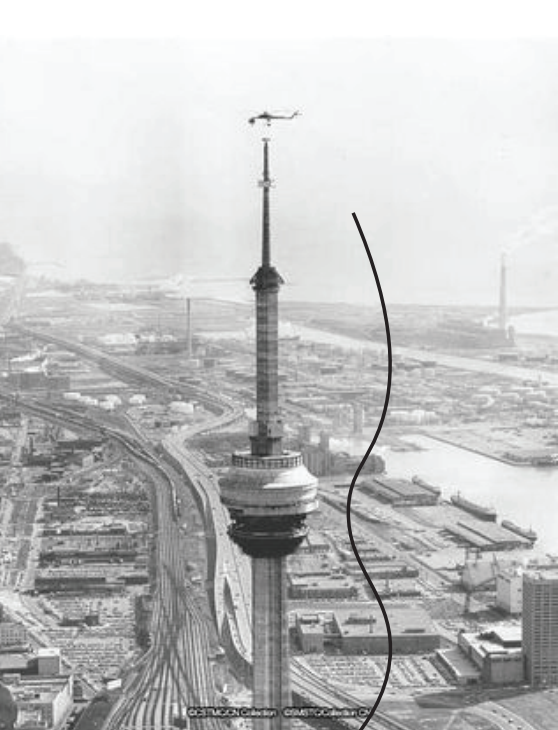
\includegraphics[width=0.25\textwidth]{A2_1.png}
    \caption{Scanned picture with a black dog hair.}
\end{figure}
You have scanned some old black-and-white photographs at home. Unfortunately a dog hair on the scanner glass has corrupted your pictures. You want to correct the picture by removing the dog hair. But first, you need to find which pixels (more accurately, chain of pixels) represent the dog hair.\\
\\
Your input is a picture $P$ of $m × n$ pixels. You are given the intensity $P(i, j)$ of each pixel $(i, j)$, which is a value of grey between 0 (black) and 1 (white). The hair is long, blackish, and at most one pixel wide. You may assume that the hair only ever passes through at most one pixel in any row of pixels. The figure above shows a hair on an old picture of the CN tower.\\
\\
The likelihood that pixel $(i, j)$ is part of the hair is given by\\
\begin{equation*}
  D_{it} =
    \begin{cases}
      0 & \text{if $P(i, j) \geq h$}\\
      1 - \frac{P(i, j)}{h} & \text{if $P(i, j) < h$}
    \end{cases}       
\end{equation*}
where $h \in (0, 1)$ is a given threshold. The idea is that any pixel lighter than $h$ is definitely not part of the hair, and pixels darker than $h$ have more probability of being part of the hair the darker they are.\\
\\
Your goal is to find a chain of pixels C. A chain is a set of pixels \{$(r, p_r) : r \in [i, j]$\} containing one pixel from every row between row $i$ and row $j$ such that for $r \in (i, j)$, pixel $p_r$ is a neighbour
of pixels $p_{r-1}$ and $p_{r+1}$. Here, we are using the standard notion of "neighbourhood" under which each pixel has at most eight neighbours (up, down, left, right, northeast, northwest, southeast, southwest). The likelihood of a chain being the hair is the sum of likelihoods of its pixels being part of the hair: $\ell (C) = \sum_{(i, j) \in C} \ell(i, j)$.
\begin{enumerate}
    \item[\textbf{(a)}] {[17 Points]} Suppose you want to compute the maximum likelihood of any chain being the hair. Use dynamic programming to design an algorithm for this.
    \begin{itemize}
        \item {[3 Points]} Clearly define the quantity that your DP is computing. (For example, in the shortest path DP that we did in class, we defined: "Let $OPT(t, i)$ be the length of the shortest path from $s$ to $t$ using at most $i$ edges.")
        \item {[5 Points]} Write a Bellman equation for this quantity, and briefly reason why your equation is correct.
        \item {[3 Points]} Write the initial conditions.
        \item {[3 Points]} What is the running time and space complexity of your algorithm (say, in a top\-down implementation)?
        \item {[3 Points]} In what order would you compute the quantities in a bottom\-up implementation? Briefly reason why this order works.
        
        \begin{mdframed}
            \textit{Solution.}\\
            
            \item[$\bullet$] Define the quantity that the DP is computing:
            \\Let $OPT(r, c)$ be the maximum likelihood of a chain being the hair start at some pixel p ends at pixel (r, c).
            \\
            \item[$\bullet$] Bellmen equation:
            \\ m: number of rows of pixels
            \\ n: number of column of pixels
            \begin{equation*}
              OPT(r, c) =
                \begin{cases}
                  0 \text{\quad\quad\quad\quad\quad\quad\quad\quad\quad\quad if $(r<0) \lor (c<0) \lor (r>m-1) \lor (c>n-1)$}\\
                  \ell(r,c) + max\{OPT(r-1, c-1), OPT(r-1, c), OPT(r-1, c+1)\} & \text{otherwise}
                \end{cases}
            \end{equation*}
            \\Assume the hair starts at some pixel $(i,k)$ and ends at $(j,l)$ where $i<j$, the maximum likelihood of a chain $OPT(j,l)$ equal to the likelihood of current pixel $\ell(j,l)$ plus maximum likelihood among 3 chains that ends at the neighbour pixel of $(j,l)$, which are $OPT(j-1, l-1)$,$OPT(j-1, l)$ and $OPT(j-1, l+1)$ based on the assumed row orientation. In this way, the problem of finding the maximum likelihood was deconstructed as finding the maximum likelihood for the neighbour pixel of current pixel plus the likelihood of the current pixel.
            \\
            \\Once the current pixel index out of bound, the recursion which represents current sub-chain ends and returns the current pixel likelihood as 0(since there is actually no pixel there).
            \\
             \item[$\bullet$] Initial condition:\\
            Base case: $OPT(r, c) = 0$ \quad if $(r<0) \lor (c<0) \lor (r>m-1) \lor (c>n-1)$
            \\
            \newpage
            \item[$\bullet$]Algorithm:
            \begin{lstlisting}
            img <- read()           # global input image
            h <- 0                  # global threshold
            m <- img.NumRows()      # number of rows
            n <- img.NumCols()      # number of columns
            M[m][n] <- 0            # global array
            
            max_likelihood(h_in)
                h = h_in                # input parameter for computing likelihood.
                max_l = 0               # maximum liklihood to be returned.
                
                for c from 0 to (n-1)               # traverse the column and 
                                                    # recursively compute maximum 
                    m_compute_opt(m-1,c)            # likelihood for each index
                    max_l = max{max_l, M[m-1][c]}   # update and record the maximum.
                return max_l
            
            m_compute_opt(i,j)
                if (i<0 || j<0 || i > m-1 || j >n-1)    # if the pixel out of bound
                        return 0                        # return likelihood 0
                                                        # (since there is no pixel).
                                                        
                if (M[i][j] is uninitialized)           # if M is not initialized 
                                                        # at current index.
                    M[i][j] <- pixel_likelihood(i,j) + max{m_compute_opt(i-1, j-1), m_compute_opt(i-1, j), m_compute_opt(i-1, j+1)}        
                                                        # initialize M[i][j].
                return M[i][j]
                
            pixel_likelihood(i,j)                       # function for calculating
                                                        # the pixel likelihood.
                if (img(i,j) < h)
                    return 1-img(i,j)/h
                return 0
            \end{lstlisting}
            \\
             \item[$\bullet$]Complexity (topdown):
            \\m: number of rows 
            \\n: number of columns
            \\
            \\Run time: O(mn)
            \\Because we only calculate the likelihood of the current pixel (i,j) if M[i][j] is uninitialized, since once we reach (i,j) we will calculate(O(1) for calculate the pixel likelihood) and initialize the optimal value at M[i][j], there are m*n pixels to reach. Hence we end up doing m*n calculations in total.
            \\
            \\Space: O(mn)
            \\Beacause we only store the maximum likelihood of the chain that ends at pixel $(i,j)$ which $0\leqi<m-1$, $0\leqj<n-1$, since there are mn value to store in total.
            \\
             \item[$\bullet$]Order of computation(bottom-up)\\
            %1 a)
            \begin{lstlisting}
            for r from 0 to m:
                for c from 0 to n:
                    compute OPT(r,c)
            \end{lstlisting}
            By this order, we actually compute all the optimal likelihood of the hair ends at $(0,0)$ to $(m-1,n-1)$. Suppose $j>i$, Since later computation $OPT(j,l)$ requires some $OPT(i,k)$, and in this order of computation guarantees that $OPT(i,k)$ has already be computed and stored since $i<j$.
        \end{mdframed}
    \end{itemize}
    \item[\textbf{(b)}] {[5 Points]} Suppose now that you actually want to find the chain with the maximum likelihood of being the hair. If there are multiple such chains, you want to return the maximum likelihood chain with the fewest number of pixels. Modify your DP so that it allows you to return the desired chain.
    \begin{mdframed}
        \textit{Solution.}\\
        %1 b)
        \\Adding a new array C[m][n] for storing chains that end/start at some index (i, j).
        \\So now we have 2 arrays of data: 
        \\1. M[i][j] store the maximum likelihood of the chain that end/start at some index (i,j)
        \\2. C[i][j] store the chains that end/start at some index (i, j).
        \\Modify m\_compute\_opt() such that if we encounter a pixel that has lower intensity than h(a pixel likely to be dog hair) add the pixel index to the current chain that locate at C[i][j], if the pixel is not a dog hair start a new chair locate at a new index $(i_{new}, j_{new})$ which keep updating by recurrence of m\_compute\_opt function.
        \\In this way, the first loop in the max\_likelihood() finishes, we get a array M that stores the maximum likelihood value of the chain start/end at each pixel index as well as a array C that stores the chain that are likely to be dog hair start/end at some index (i, j).
        \\So the second loop in max\_likelihood() traverse each index of array C, if C[i][j] is initialized(indicate that there is a chain start/end here), compare M[i][j] with the maximum value we get from first loop, if M[i][j] is the maximum value with minimum chain size, then return the chain C[i][j] as result.
        
        \begin{lstlisting}
        img <- read()           # global input image
        i_c <- 0                # global row index for array C
        j_c <- 0                # global column index for array C
        h <- 0                  # global threshold
        m <- img.NumRows()      # number of rows
        n <- img.NumCols()      # number of columns
        C[m][n] <- 0            # global chain array
        M[m][n] <- 0            # global likelihood array
        
        max_likelihood(h_in)
                h = h_in                # input parameter h
                max_l = 0               # maximum likelihood of the chains
                result = {}             # result chain to be returned
                len = INF               # initialize length to infinity
                for c from 0 to (n-1)
                    i_c = m-1           # initialize the moving index of C   
                    j_c = c             # initialize the moving index of C
                    m_compute_opt(m-1,c)
                    max_l = max{max_l, M[m-1][c]}
                
                for r from o to (m-1)
                    for c from 0 to (n-1)
                        if (C[r][c] is initialized 
                                && M[r][c] == max_l 
                                && C[r][c].length < len)
                            # if there is a chain and the chain is the shortest 
                            # one with the maximum likelihood, it is the desired chain.
                            result = C[r][c]
    
                return result
                
        m_compute_opt(i,j)
                if (i<0 || j<0 || i > m-1 || j >n-1)
                        return 0
                if (pixel_likelihood(i,j) >= h)     # if we encounter a pixel 
                                                    # that is not dog hair, update
                                                    # the index to a new 
                                                    # start/end location
                    i_c = i
                    j_c = j
                else
                    C[i_c][j_c].add((i,j))          # if the pixel is still dog hair,
                                                    # add it to the current chain.
                if (M[i][j] is uninitialized)
                    M[i][j] <- pixel_likelihood(i,j) + max{m_compute_opt(i-1, j-1), m_compute_opt(i-1, j), m_compute_opt(i-1, j+1)}
                return M[i][j]
        \end{lstlisting}
        
        
    \end{mdframed}
    \item[\textbf{(c)}] {[3 Points]} (Open Ended Question) Is the likelihood function ($\ell (i, j)$ and $\ell (C)$) well-designed in your opinion? Describe a type of image on which this algorithm would perform poorly for the ultimate objective of finding the hair. Suggest a modification to the likelihood formula that you think might perform better.
    \begin{mdframed}
        \textit{Solution.}\\
        %1 c)
        The likelihood function $\ell(i,j)$ is not well-designed. The algorithm with original likelihood function would perform poorly because this likelihood only provide an upper bound h and if $P(i,j) < h$ satisfies, then the darker the pixel is the higher likelihood it gets.
        \\
        \\If there is a completely black image which has a blackish(but not completely black) dog hair locate at the center of the image. The algorithm with the original likelihood function would not work since the completely black pixel always has highest likelihood. 
        \\
        \\I suggest using a normal distribution as the likelihood function:
        \\By adjusting parameters $\mu$ and $\sigma$:
        \\
        \\$\ell(i,j)=\frac{1}{\sqrt{2\pi\sigma^2}}e^{-\frac{(P(i,j)-\mu)^2}{2\sigma^2}}$
        
        
    \end{mdframed}
\end{enumerate}
\subsection*{Q2 [20 Points] Approximating Functions}
You are given $n + 1$ points \{$p_0, p_1, ..., p_n$\}, where $p_i = (x_i, y_i)$ for $0 \leq i \leq n$. The points are sorted in the increasing order of (unique) $x_i$’s: that is, $x_0 < x_1 < ... < x_n$.\\
\\
In reality, these are sample points on the curve of some unknown function $f: \mathbb{R} \rightarrow \mathbb{R}$ with $y_i = f(x_i)$ for each $0 \leq i \leq n$. Your goal is to approximate this function using a sequence of line segments.\\
\\
If you use the sequence of $n$ line segments joining all adjacent points (i.e. joining $p_i$ and $p_{i+1}$ for $0 \leq i < n$), then this provides an excellent approximation since it passes through $(x_i, y_i)$ for each
$0 \leq i \leq n$. However, it uses too many line segments.\\
\\
If you replace the line segments between $p_i$ and $p_j$ (where $j > i$) with a single straight line connecting $p_i$ and $p_j$, then the error introduced is given by
\[E[i, j] = \sum_{\ell = i + 1}^{j - 1} |y_{\ell} - \hat{y_{\ell}}|,\]
where $(x_{\ell}, \hat{y_{\ell}})$ is point through which the line segment joining $p_i$ and $p_j$ passes. Note that $E[i, i+1] = 0$ for all $i$.\\
\\
Suppose every line segments costs $C$. If you select a subset of points (without changing their order) $(p_{i_0},...,p_{i_k})$ and use the $k$ line segments connecting adjacent points $p_{i_m}$ and $p_{i_{m+1}}$ for $0 \leq m < k$, the total error of this approximation is $\sum_{m=0}^{k}E[i_m, i_{m+1}] + k \cdot C$. Your goal is to find the optimal approximation which minimizes this error. Note that $k$ is not given to you. You need to optimize
the number of line segments to use too. See Figure for an illustration of the problem.\\
\begin{figure}[H]
    \centering
    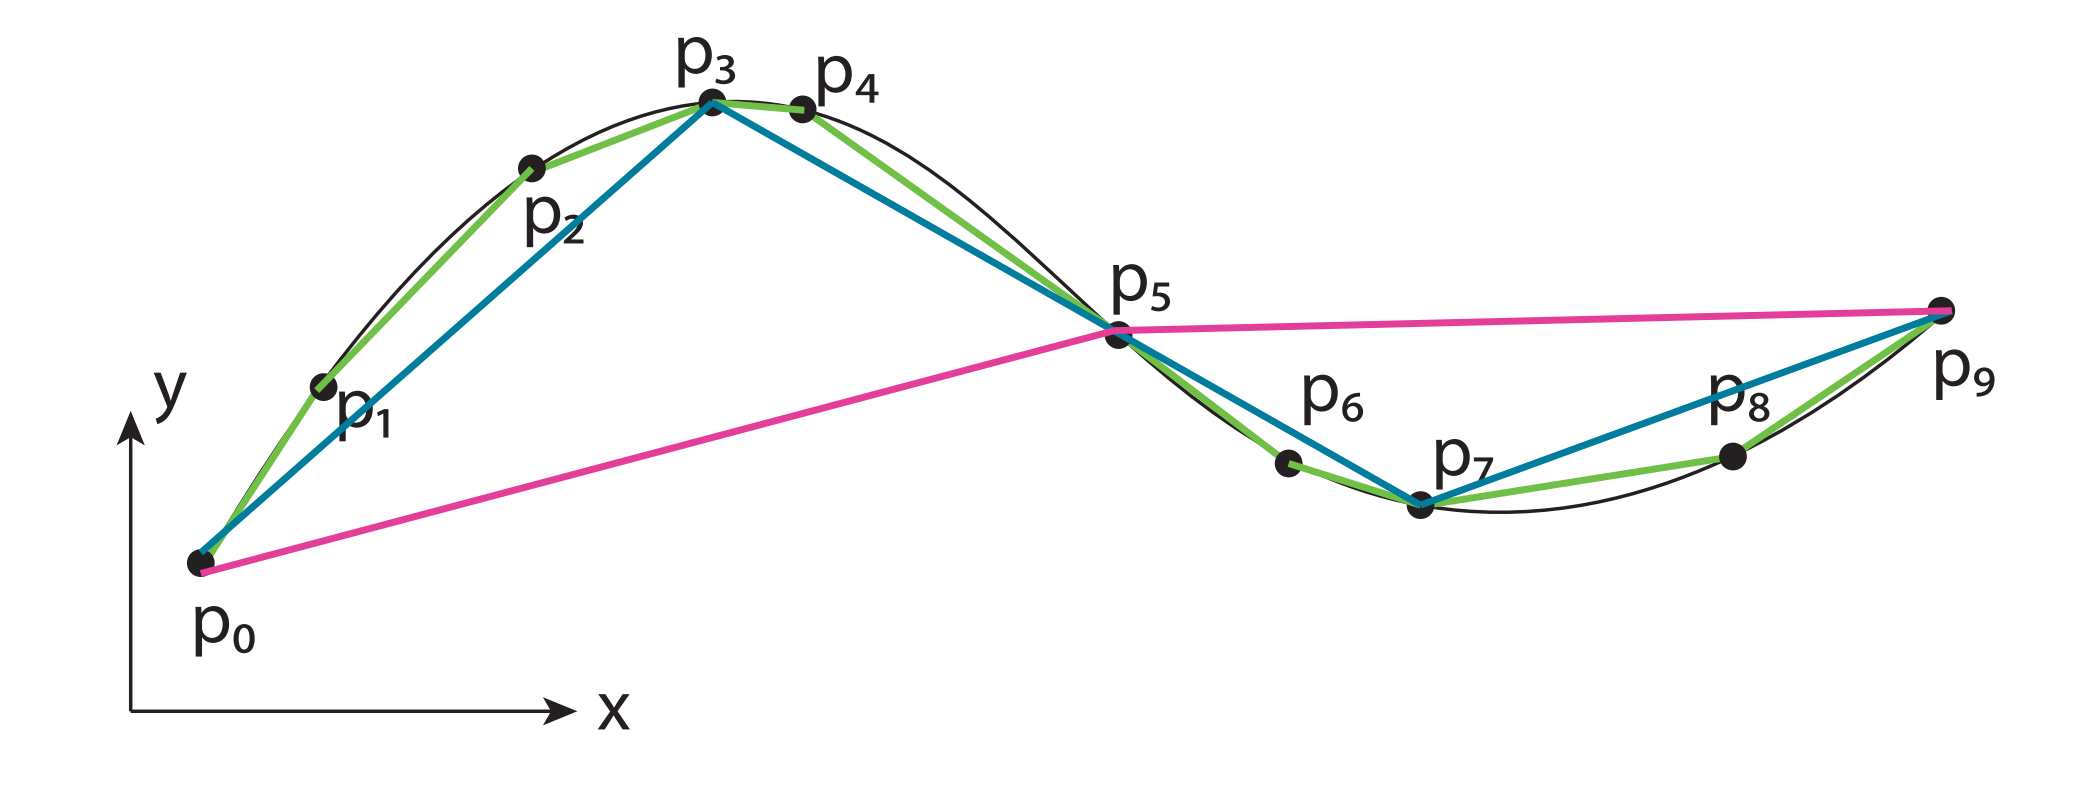
\includegraphics[width=0.85\textwidth]{A2_2.png}
    \caption{The function (black curve) with samples $p_0, ..., p_9$ is shown approximated using 9 (green), 3 (blue), and 2 (pink) line segments. The optimal approximation will try to use fewer line segments but also try to achieve a low approximation error.}
\end{figure}

\begin{enumerate}
    \item [\textbf{(a)}] {[3 Points]} Express the total error of an approximation \{$p_{i_0}, ... ,p_{i_k}$\} explicitly in terms of the inputs to the problem ($(x_i, y_i)$ for $0 \leq i \leq n$).
    \begin{mdframed}
        \textit{Solution.}\\
        %2 a)
        Let the set of points selected for approximation be $S = \{p_{i_0}, ..., p_{i_k}\}$, the total error of this approximation is
        \begin{align*}
            TotalError(S) &= \sum_{j = 0}^{k - 1} E[i_j, i_{j + 1}] + k \cdot C\\
            &= \sum_{j = 0}^{k - 1} \Bigg[\sum_{\ell = j}^{j + 1} |y_{i_{\ell}} - \hat{y_{i_{\ell}}}| \Bigg] + k \cdot C
        \end{align*}
        The approximation $\hat{y_{\ell}}$ is
        \[\hat{y_{i_{\ell}}} = k \cdot x_{i_{\ell}} + b, x_{i_{\ell}} \in [x_{i_j}, x_{i_{j + 1}}], y_{i_{\ell}} \in [y_{i_j}, y_{i_{j + 1}}]\]
        By the slope equation,
        \[k = \frac{y_{i_{j + 1}} - y_{i_j}}{x_{i_{j + 1}} - x_{i_j}}\]
        When $x_{i_{\ell}} = x_{i_{j + 1}}$, $\hat{y_{i_{\ell}}} = y_{i_{j + 1}}$, then
        \[y_{i_{j + 1}} = \frac{y_{i_{j + 1}} - y_{i_j}}{x_{i_{j + 1}} - x_{i_j}} \cdot x_{i_{j + 1}} + b\]
        \[b = \frac{x_{i_{j + 1}}y_{i_j} - x_{i_j}y_{i_{j + 1}}}{x_{i_{j + 1}} - x_{i_j}}\]
        Thus
        \[TotalError(S) = \sum_{j = 0}^{k - 1} \Bigg[\sum_{\ell = j}^{j + 1} |y_{i_{\ell}} - \frac{y_{i_{j + 1}} - y_{i_j}}{x_{i_{j + 1}} - x_{i_j}} \cdot x_{i_{\ell}} - \frac{x_{i_{j + 1}}y_{i_j} - x_{i_j}y_{i_{j + 1}}}{x_{i_{j + 1}} - x_{i_j}}| \Bigg] + k \cdot C\]
    \end{mdframed}
    \item [\textbf{(b)}] {[17 Points]} Describe a dynamic programming solution that finds the optimal subset of points \{$p_{i_0}, p_{i_1}, ..., p_{i_k}$\} minimizing the total error.
    \begin{mdframed}
    Before the following discussion, the algorithm is presented here in the pseudo code form for convenience of explanation. Also, based on the final sub-part of part b), a bottom-up algorithm is implemented. In the algorithm below, $n$ stands for the index of the end point of the curve (i.e., $p_n$), $i, \; j$ stands for $\beta, \; \gamma$ respectively, \texttt{segmentCost} stands for $C$ and Error stands for $E$ by the definition of the problem and Bellman equation below.\\
    \\
    \textbf{Algorithm:}
     \lstset{language=C}
    \begin{lstlisting}
typedef struct {
    double opt;
    double* selectedPoints;
} Result;

Result Bottom_Up-DP(int n, double segmentCost) {
    // memoization list to store the minimum total error of the sub-problems.
    double M[n + 1];
    // a list to store the solution
    // the number j at index i stands for the start point p_j such that j < i
    // and <p_j, p_i> is a line segment involving the approximation
    double S[n + 1];
    for (int i = 0; i <= n; i++) {
        if (i == 0) { //base cases
            // the end point is always in the solution, put this end point
            // at first location (i.e., indexed with 0), which is used not 
            // for  p_1,...,p_n  to set the start point for the line
            // segment that ends with them except for n = 0
            S[i] = n;
            // there is no error if there is only one single point
            M[i] = 0;
        } else {
            double q = INFINITY;
            for (int j = 0; j < i; j++) {
                double error = Error(j, i) + segmentCost + M[j];
                if (q > error) {
                    q = error;
                    S[i] = j;
                }
            }
            M[i] = q;
        }
    }
    
    Result result;
    result.opt = M[n];
    result.selectedPoints = S;
    return result;
}

// not a part of algorithm, just used to show the solution
void print_result(int n, double segmentCost) {
    Result result = Bottom_Up_DP(n, segmentCost);
    double* solution = result.selectedPoints;
    
    printf("%lf", solution[0]);
    while (n > 0) {
        printf("%lf ", solution[n]);
        n = n - solution[n];
    }
}
    \end{lstlisting}
    \end{mdframed}
    \begin{itemize}
        \item {[3 Points]} Clearly define the quantity or quantities that your DP is computing.
        \begin{mdframed}
            \textit{Solution.}\\
            %2 b)
            This algorithm works to find a strictly-ordered set subset of points \{$p_{i_0}, ..., p_{i_{\alpha}}$\}, $0 \leq \alpha \leq k$ which optimizes the approximation with minimum total error from a strictly-ordered set \{$p_0, ..., p_{\beta}$\}, $0 \leq \beta \leq n$ while $p_i = (x_i, y_i)$ and $x_0 < x_1  ... < x_n$, $x_0 \leq x_{\beta} \leq x_n$ to minimize the total error.\\
            \\
            Let $OPT(\beta)$ denotes the minimal total error and $S(\beta)$ denotes the set of points that approximize the curve optimally if selecting points \{$p_{i_0}, ..., p_{i_{\alpha}}$\} from \{$p_0, ..., p_{\beta}$\}, while $p_{i_0} = p_0$ and $p_{i_{\alpha}} = p_{\beta}$ trivially, since the group of the approximation line segments of a curve always start at the initial point of the curve and the end point of the curve, let $1 \leq \gamma \leq \beta, \; p_{\gamma} \in \{p_0, ..., p_{\beta}\}$. \underline{Then the quantity this algorithm is computing is $OPT(n)$ and $S(n)$.} Also, based on the problem, $C$ is the cost of the line segment connected between $P_{\gamma}$ and $P_{\beta}$, $E(\gamma, \; \beta)$ is the error of this line segment.
        \end{mdframed}
        \item {[5 Points]} Write a Bellman equation for these quantities, and briefly reason why your equation is correct.
        \begin{mdframed}
            \textit{Solution.}\\
            %2 b)
            Bellman equation:
            \begin{equation*}
              OPT(\beta) =
                \begin{cases}
                  0 & \text{if $\beta = 0$}\\
                  \min_{1 \leq \gamma \leq \beta}(E(\gamma, \; \beta) + C + OPT(\gamma)) & \text{if $0 < \beta \leq n$}
                \end{cases}       
           \end{equation*}
           
           \begin{equation*}
              S(\beta) =
                \begin{cases}
                  \{n\} & \text{if $\beta = 0$}\\
                  S(\gamma + 1) & \text{if $\beta > 0 \wedge E(\gamma, \; \beta) + C + OPT(\gamma) \geq OPT(\gamma + 1)$}\\
                  \{\gamma\} \cup S(\gamma) & \text{if $\beta > 0 \wedge E(\gamma, \; \beta) + C + OPT(\gamma) < OPT(\gamma + 1)$}
                \end{cases}       
           \end{equation*}
           The algorithm works like the following:
           \begin{itemize}[leftmargin=20.7mm]
               \item[\textbf{Base Case:}] $\beta = 0.$
               \begin{itemize}
                   \item[\textbf{OPT:}] The algorithm reaches a single point (the point is the start point of the curve), then there is no error since a point is not a line segment, hence a vacuous result is returned, which is 0.
                   \item[\textbf{S:}] The algorithm starts finding the optimal solution at the end point of the curve, which is $p_n$. Therefore, the first point set formed contains n.
               \end{itemize}
               \item[\textbf{Otherwise:}] $\beta \in [1, n].$
               \begin{itemize}
                   \item[\textbf{OPT: }] The algorithm is searching a line segment such that $p_{start} \in \{p_0, ..., p_{\beta - 1}\}$ and $p_{end} = p_{\beta}$ (i.e., the last line segment of the set of choices of line segments). Denote the $p_{start}$ by $p_{\gamma}$, a point between $p_0$ inclusive and $p_{\beta}$ exclusive. Denote this line segment by $\overrightarrow{p_{\gamma}p_{\beta}}$. Since the equation of an error for such a line segment is $E(\gamma, \; \beta)$, also the cost $C$ should be taken into consideration, hence the error for $\overrightarrow{p_{\gamma}p_{\beta}}$ is $E(\gamma, \; \beta) + C$. Since the minimum total error is sum of the error of the optimal selection of $p_{\gamma}$ regarding $p_{\beta}$ and the minimum total error from the points ahead of $p_{\gamma}$, including $p_{\gamma}$ (i.e., $p_0, ..., p_{\gamma}$), then the algorithm works recursively to find the optimal solution in the subset \{$p_0, ..., p_{\gamma}$\}, thus the recursive equation should be defined as: $\min_{1 \leq \gamma \leq \beta}(E(\gamma, \; \beta) + C + OPT(\gamma)$. Therefore the equation correctly describe this algorithm.
                   \item[\textbf{S: }] There are two cases while searching each $\gamma \in [0, \; \beta)$:
                   \begin{itemize}
                       \item $\gamma$ is not in the optimal solution.\\
                        Since all points are strictly ordered, and this algorithm confirms the start point of a line segment in the optimal approximation which ends with given $\beta$ by searching from left to right, thus $\gamma$ starts at 0 and ends with a point left-neighbouring $p_{\gamma}$. Therefore, if $p_{\gamma}$ is not in optimal solution, searches $p_{\gamma + 1}$, the point in the right hand side of $p_{\gamma}$.\\
                       \item $\gamma$ is in the optimal solution.\\
                       If the $p_{\gamma}$ is searched and this point is the one in the optimal solution, then $\gamma$ is put into the solution, and this solution is unioned with the solution of the sub-problem $\{p_0, ..., p_{\gamma - 1}\}$. Therefore, the equation $S(j)$ correctly describes the algorithm.
                   \end{itemize}
               \end{itemize}
           \end{itemize}
        \end{mdframed}
        \item {[3 Points]} Write the initial conditions.
        \begin{mdframed}
            \textit{Solution.}\\
            %2 b)
            $OPT(0) = 0$.\\ This means the algorithm is computing the minimal error for a line segment starts and ends at $p_0$, which means there is no line segment. Trivially, the error is 0.\\
            $S(0) = \{n\}.$\\
            This means the algorithm is searching the end point of the curve, which is also always the last point of the approximation line segments. Thus, the first search returns a set contains the end point of the curve, $\{n\}$.
        \end{mdframed}
        \item {[3 Points]} What is the running time and space complexity of your algorithm (say, in a top-down implementation)?
        \begin{mdframed}
            \textit{Solution.}\\
            \textbf{Time Complexity:}\\
            Time to compute the error of one pair: $O(1)$\\
            Number of pairs: $\sum_{i = 1}^{n} i = \frac{(n + 1) \cdot n}{2} \in O(n^2)$\\
            Total time to compute error: $O(1) \cdot O(n^2) = O(n^2)$\\
            Loop through each point to check the minimum total error: $O(n)$, which means there are $O(n)$ calls to compute the minimum total error.\\
            Each computation takes $O(n)$ time.\\
            Thus the total running time for DP with error known is $O(n) \cdot O(n) = O(n^2)$\\
            Time Complexity $= O(n^2) + O(n^2) = O(n^2)$.\\
            \\
            \textbf{Space Complexity:}\\
            Space to store the minimum total error for a sub-problem ends with each point (i.e., length of $M$, which memorizes $OPT(i)$): $O(n)$\\
            Space to store the optimal points selection that end with each point (i.e., length of $S$, which memorizes $S(i)$): $O(n)$\\
            Space Complexity = $O(n) + O(n) = O(n)$
            %2 b)
        \end{mdframed}
        \item {[3 Points]} In what order would you compute the quantities in a bottom-up implementation? Briefly reason why this order works.
        \begin{mdframed}
            \textit{Solution.}\\
            %2 b)
            Except for the base case that the algorithm puts the end point $p_n$ of this approximation at the left-most side of the solution array, this algorithm computes the quantities from start point $p_0$ to the end point $p_n$.\\
            \begin{proof}
            The proof is constructed by strong induction.\\
            \textbf{Base case:} $i = 0$.\\ The algorithm is searching the optimal point ahead of $p_0$ to minimizes the total error, in which the algorithm returns 0 as minimum total error because a single point does not make a line segment. Also, since there is no point ahead of $p_0$, a trivial solution, $\{n\}$, which is the end point is returned (in case of there is only one point, then end point is $p_0$).\\
            \textbf{Inductive Hypothesis:} Suppose $S(i)$ gives optimal selection for each point and $OPT(i)$ gives the minimum total error, $0 \leq i \leq n - 1$. Prove $S(n)$ and $OPT(n)$ produces expected result as well.\\
            \textbf{Inductive step:}
            Since $p_n$ is the end point, it is always in the optimal solution set. Thus there exists a point $p_{\gamma}$ such that $0 \leq \gamma \leq n - 1 < n$ to construct a line segment with $p_n$, $\overrightarrow{p_{\gamma}p_n}$ that minimizes the error, consisting of the optimal solution $S(n) = S(\gamma) \cup \{\overrightarrow{p_{\gamma}p_n}\}$. By the induction hypothesis, $S(\gamma)$ contains the optimal solution for all points $\{p_0, ..., p_{\gamma}\}$, which means $M[\gamma]$ also minimizes the total error of the sub-problem, $\overrightarrow{p_{\gamma}p_n}$ also minimize the error, thus the total error $M[n] = E[\gamma, \; n] + C + M[\gamma]$, is minimized by $S(n)$ as wanted.
            \end{proof}
        \end{mdframed}
    \end{itemize}
    You will get the 17 marks for part (b) if you describe an $O(n^3)$ time algorithm. You will get 5 bonus marks if your solution works in $O(n^2)$ time.
\end{enumerate}

\subsection*{Q3 [30 Points] Maximum Flow}
Suppose you are given a network $N$, a maximum flow $f$ on $N$, and one edge $e_0 \in N$ such that $f(e_0) = c(e_0)$. You are also given that $f$ has \textit{integer} flow values $f(e)$ for all edges $e$.
\begin{enumerate}
    \item [\textbf{(a)}] {[5 Points]} If we decrease $c(e_0)$ by 1 (i.e., let $c'(e_0) = c(e_0) − 1$ but other capacities remain the same), then one might expect that the maximum flow on $N$ might also decrease by one unit. But does this always happen?\\
    \\
    Either give a specific example where the maximum flow on $N$ does not change (and show that this is the case), or give a general argument that the maximum flow on $N$ always changes.
    \begin{mdframed}
        \textit{Solution.}\\
        \textbf{For first case, the maximum flow does not change:}\\
        The edge between B and D is $e_0$ and the maximum flow remains 10\\
        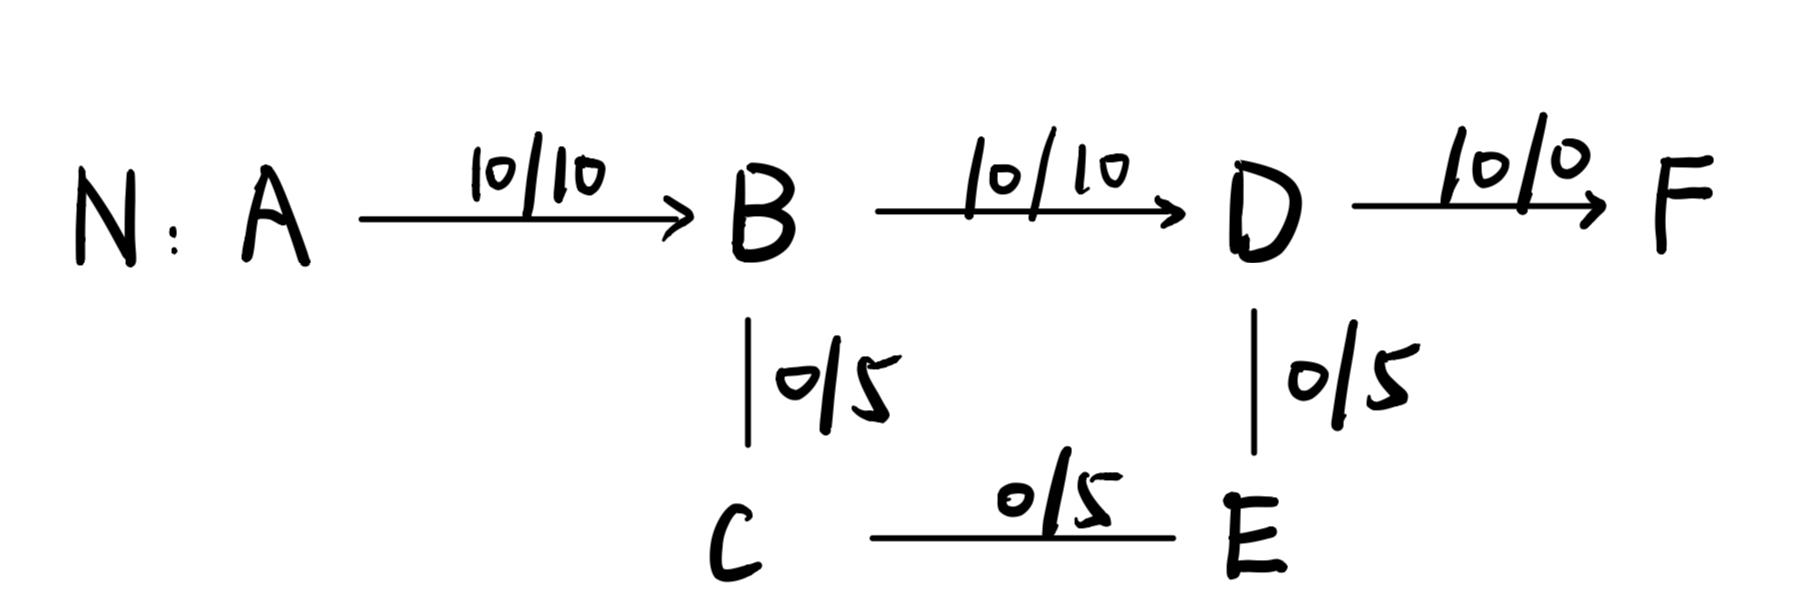
\includegraphics[scale= 0.12]{hw2/N.jpg}
        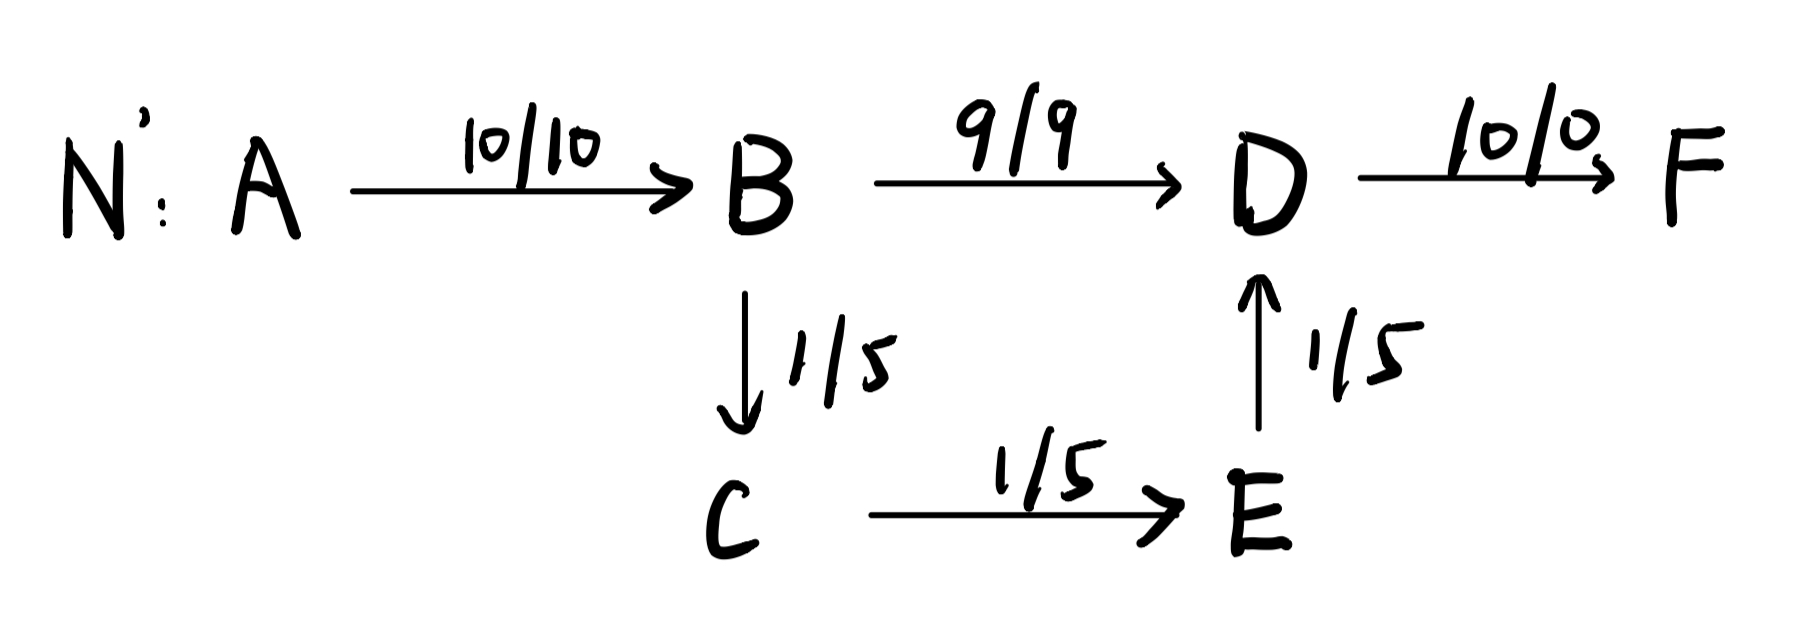
\includegraphics[scale= 0.12]{hw2/N1.jpg}\\
        \textbf{Second Case where the maximum flow on N changes:}\\
        if $e_0$ is in the minimum cut (A,B), then if we decrease $c(e_0)$ by 1, the sum of capacities of edges leaving A will decrease by 1 unit. The maximum flow on N always changes.
    \end{mdframed}
    \item[\textbf{(b)}] {[10 Points]} Irrespective of your answer on the previous part, there are cases when this change in capacity causes the maximum flow to decrease.\\
    \\
    Give an efficient algorithm that takes a network $N$, a maximum integral flow $f$ on $N$, and one edge $e_0 \in N$ such that $f(e_0) = c(e_0)$ and that determines a new maximum flow in the network $N'$, where $N' = N$ except for $c'(e_0) = c(e_0) - 1$.\\
    \\
    Include a brief justification that your algorithm is correct and a brief analysis of your algorithm’s worst-case runtime (which should be as small as possible).
     \begin{mdframed}
        \textit{Solution.}\\
        \textbf{Algorithm:}\\
        Assuming that $e_0 = (u,v)$ and flow is starting from s, ending at t. after decreasing $c(e_0)$ by 1.\\ Firstly we need to send one unit back from t to s through $e_0$ in the network N, then using breath first search to find the shortest augmenting path on new created network $N$. If there exits such an augment path that means we can add one more unit on this path and it will remain the maximum flow f. if there is no such a augmenting path, it means that the maximum value will be $f-1$\\
        \textbf{Correctness:}\\
        After we send back one unit from s to t through $e_0$ based on network N, it will make the flow feasible according to the current capacity on $e_0$.\\
        And it is obvious that there is an augmenting path from s to u and an augmenting path from v to t. If there is no augmenting path found by breath first search, it means we cannot add more flow unit on the path from u to v, the current flow is maximal, then it is $f-1$. Otherwise, because of the integer flow values, the $bottleneck \geq 1$. we can add at most one unit on this path, because only one remaining capacity on the path from s to u and v to t. And maximum value of flow will stay at $f$.\\
        \textbf{Complexity:}\\
        Decreasing one unit from t to s takes $O(V)$ time, Where V is the number of vertices. And it uses polynomial time $O(E)$ to find augmenting path by breath first search, Where E is the number of edges. Optionally, it takes $O(V)$ to augment the path. The total time is $O(V+E)$.
    \end{mdframed}
    \item[\textbf{(c)}] {[5 Points]} If we increase $c(e_0)$ by 1 (i.e., let $c'(e_0) = c(e_0) + 1$ but other capacities remain the same), then one might expect that the maximum flow on $N$ might also increase by one unit. But does this always happen?\\
    \\
    Either give a specific example where the maximum flow on $N$ does not change (and show that this is the case), or give a general argument that the maximum flow on $N$ always changes.
    \begin{mdframed}
        \textit{Solution.}\\
        \textbf{First case where the maximum flow on N does not change:}\\
        The edge between B and C is $e_0$ and the maximum flow remains 10\\
        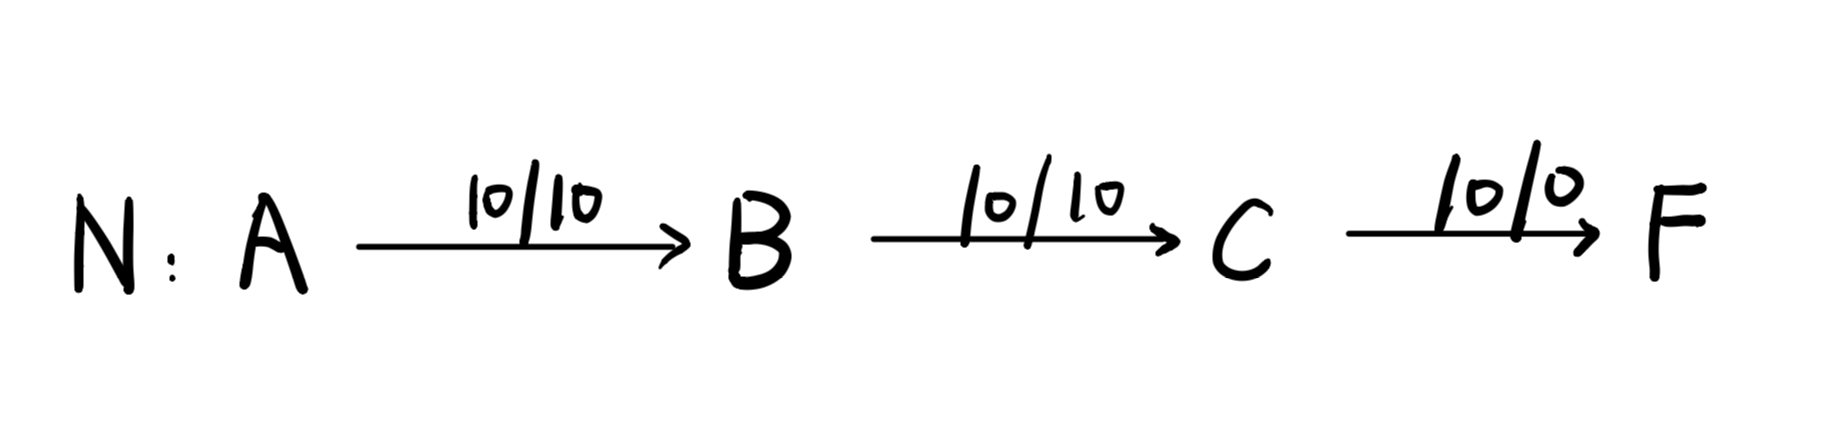
\includegraphics[scale=0.1]{hw2/incre_N0.jpg}
        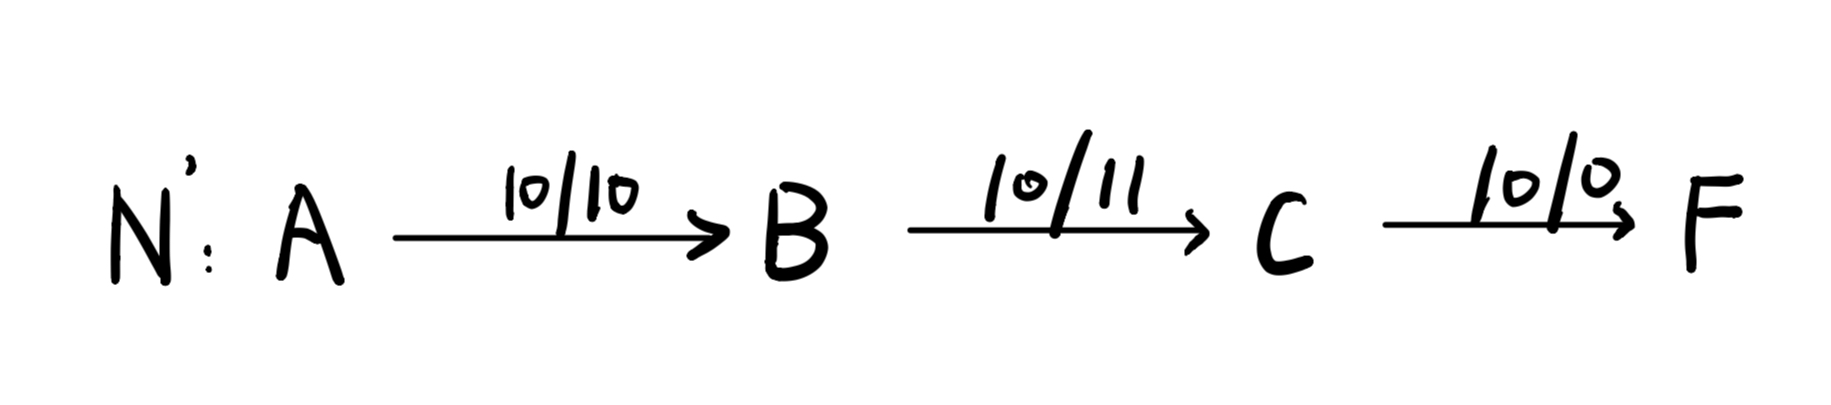
\includegraphics[scale=0.1]{hw2/incre_N.jpg}\\
        \textbf{Second Case where the maximum flow on N' changes:}\\
        if $e_0$ is in the minimum cut (A,B), then if we increase $c(e_0)$ by 1, the sum of capacities of edges leaving A will increase by 1 unit. The maximum flow on N always changes.
    \end{mdframed}
    \item[\textbf{(d)}] {[10 Points]} Irrespective of your answer on the previous part, there are cases when this change in capacity causes the maximum flow to increase.\\
    \\
    Give an efficient algorithm that takes a network $N$, a maximum integral flow $f$ on $N$, and one edge $_0 \in N$ such that $f(e_0) = c(e_0)$ and that determines a new maximum flow in the network $N'$, where $N' = N$ except for $c'(e_0) = c(e0) + 1$.\\
    \\
    Include a brief justification that your algorithm is correct and a brief analysis of your algorithm’s worst-case runtime (which should be as small as possible).
    \begin{mdframed}
        \textit{Solution.}\\
        \textbf{Algorithm:}\\
        After increasing $c(e_0)$ by 1, using breath first search to find the shortest augmenting path which contains $e_0$ on network $N'$.\\
        For the first case, if we can't find such a augmenting path containing $e_0$, it means that the maximum flow on network $N'$ will be same as the previous f on $N$.\\
        For the second case, if we can find such a augmenting path, and the flow on edge $e_0$ is still $f(e_0)$ with capacity $f(e_0)+1$, Because it is an integer flow, we have the the $bottleneck \geq 1$. Therefore, we are able to sending one unit of flow along path, then $f(e_0) = c(e_0)$. The maximum flow in the network $N'$ is $f+1$.\\
        \textbf{Correctness:}\\
        if these are cases when the change in capacity causes the maximum flow to increase, we have known that the minimum capacity of any cut in network N is equal to maximum flow f, the min cap in $N'$ should be at most $f+1$ because $N' = N$ except for $c'(e_0) = c(e_0) + 1$. Therefore, after we add one more unit of flow in the path, by the max flow-min cut theorem, the max flow is equal to capacity of the minimum cut and is $f+1$.\\
        \textbf{Complexity}\\
        For the worst case, it uses polynomial time $O(E)$ to find shortest augmenting path by breath first search, where E is the number of edges. And it takes $O(V)$ to augment the path, where V is the number of vertices\\
        The total time is $O(E+V)$
    \end{mdframed}
\end{enumerate}
\section*{BONUS QUESTION}
{\fontsize{13}{14} \selectfont \textbf{Q4 [15 Points] Bloober}  (Remember: $20\%$ rule does not apply to this bonus question)}\\
A start-up in the competitive self-driving bus ride sharing space, Bloober, would like to figure out the minimum number of buses it needs in its fleet to service the $n$ routes: each route $r_i$ departs from bus stop $s(r_i)$ at time $d(r_i)$ and ends at stop $e(r_i)$. The travel time between any two bus stops $a$ and $b$ is $t(a, b)$.\\
\\
Note that we only care about the start stop, the end stop, and the travel time $t(s(r_i), e(r_i))$ of going from the start stop to the end stop. We do not care about any stops in between.\\
\\
A bus that is not in use (after it has reached the end stop of its current route) can be used to service another route if it can reach the start stop of that route by the scheduled departure time of that route.
\begin{enumerate}
    \item [\textbf{(a)}] {[8 Points]} Design an algorithm that can test if Bloober can service the routes using exactly $k$ buses. You get 4 marks for describing the algorithm, and 4 marks for proving its correctness.\\
    \\
    You can assume that each bus can reach the start stop of the first route that it services by the departure time of that route, and once a bus reaches a stop, it is allowed to just stay there for a while. Note thus that you can trivially service $n$ routes with $n$ buses. The goal is clearly to service them with a smaller number of buses by reusing buses to service multiple routes where the travel times are compatible.
    \begin{mdframed}
        \textit{Solution.}\\
        %4 a)
        \item[$\bullet$] Algorithm:
        \\Say route $r_j$ is \textbf{compatible} with $r_i$ for $i \neq j, 0 \leq i,j <n$, if the bus which finishes $r_i$ can still go to the start stop of $r_j$ before the departure time $d(r_j)$ of route $r_j$.
        \\
        \\To test whether there is a feasible schedule using k buses:
        \\Construct a network N based on input k:
        \\\textbf{Vertices:} 
        \\- All start stops $s(r_i)$ and end stops $e(r_i)$ for all route $r_i$, $0\leq i<n$.
        \\- Source vertex s has demand -k.
        \\- Sink vertex t has demand k.
        \\\textbf{Edges:} 
        \\- For each route $r_i, 0\leq i < n$, there is a edge $e_{ri}$ that connects the start stop $s(r_i)$ and end stop $e(r_i)$ with lower bound 1 and capacity 1.
        \\- For each route $r_i, 0\leq i < n$, for all routes $r_j, j \neq i, 0\leq j < n$ if $r_j$ are compatible with $r_i$, then there are edges $e_{ij}$ connect from $e(r_i)$ to $s(r_j)$ with lower bound 0 and capacity 1.
        \\- There are edges $e_{si}$ from source vertex s connect to every start stop $s(r_i)$ for all route $r_i, 0\leq i <n$, with lower bound 0 and capacity 1.
        \\- There are edges $e_(ei)$ from each end stop $e(r_i), 0\leq i <n$ to the sink vertex t, with lower bound 0 and capacity 1.
        \\- There is a edge $e_(st)$ connects source vertex s and sink vertex t with lower bound 0 and capacity k.
        \\
        \\Applying Ford-Fulkerson algorithm on network N to get a circulation f.
        \\Loopting through circulation f:
        \\(1) For each edge e, the flow of e is within its lower bound and capacity.
        \\(2) For each vertices, the demand of each vertices is the amount of flow going out of this vertex minus the amount of flow going in.
        \\If both of (1) and (2) satisfies, then f is a valid circulation.
        \\If f is a valid circulation, then Blooper can service the routes using exactly k buses, otherwise it cannot.
        
        \\
        \item[$\bullet$] Proof of correctness:
        \\By contradiction,
        \\Assume that if it doesn't have a feasible circulation with k buses and the Bloober can still service the routes using exactly k buses.
        \\By the assumption that it is not a feasible circulation which means that either conditions (1) or (2) from above algorithm fails. 
        \\However, 
        \\- if (1) fails, then there is a edge has flow is not within its lower bound and capacity, which means that there is route $r_i$ is out of service, it contradicts that Bloober can service the routes using k buses.
        \\- if (2) fails, then there is a vertex that demand of each vertices is not equal to the amount of flow going out of this vertex minus the amount of flow going in. This is also a contradiction.
        \\Therefore, the algorithm is correct.
    \end{mdframed}
    \item[\textbf{(b)}] {[4 Points]} What is the time complexity of your algorithm, assuming the Na\"ive implementation of the Ford Fulkerson algorithm that runs in $O(mnC)$ time, where $m$, $n$, and $C$ are the number of edges, the number of vertices, and the sum of capacities of edges from the source vertex, respectively.
     \begin{mdframed}
        \textit{Solution.}\\
        %4 b)
        \item[$\bullet$] Complexity:
        \\n: the number of stops
        \\m = $n^2$: number of edges
        \\C = n: the sum of capacities of edges from the source vertex
        \\Since the Ford Fulkerson algorithm runs in O($n^4$) in this network,
        \\Creating the network N is O($n^2$),
        \\Looping through each vertices and edges to test feasibility is O($n^2$),
        \\Hencce the overall complexity is O($n^4$)
        
    \end{mdframed}
    \item[\textbf{(c)}] {[3 Points]} Use the solution to part (a) to determine the minimum number of buses needed in the fleet. What is the time complexity of the overall algorithm?
     \begin{mdframed}
        \textit{Solution.}\\
        %4 c)
        \begin{lstlisting}
            low <- 0
            hi <- n
            k <- 0
            
            get_circulation(k_in)
                # ceate the network and get the circulation
            
            test_feasibility(f)
                # looping through circulation f and return whether it is a feasible circulation
                # return true if it is feasible, otherwise false
            
            cal_min_k(l,h)
                k <- (l + h)/2
                f <- get_circulation(k)

                if (test_feasibility(f))
                    if (l == h)
                        return k
                    cal_min_k(l, k)
                else 
                    if (l == h)
                        return k+1
                    cal_min_k(k, h)

            main()
                return get_min_k(low, hi)
        \end{lstlisting}
        \\Since we basically using binary search to find k which is $O(logn)$
        \\The complexity for algorithm in (a) is $O(n^4)$ from (b)
        \\The overall complexity is $O(n^4logn)$
    \end{mdframed}
\end{enumerate}
\end{document}